\begin{frame}[fragile]\frametitle{}
\begin{center}
{\Large Singular Value Decomposition (SVD)}
\end{center}
\end{frame}


%%%%%%%%%%%%%%%%%%%%%%%%%%%%%%%%%%%%%%%%%%%%%%%%%%%
\begin{frame}[fragile]
\frametitle{Singular Value Decomposition}

\begin{itemize}
	\item Dimension reduction by Matrix Decomposition
	\item Another way to do PCA
\end{itemize}
\end{frame}

%%%%%%%%%%%%%%%%%%%%%%%%%%%%%%%%%%%%%%%%%%%%%%%%%%%
\begin{frame}[fragile]
\frametitle{Singular Value Decomposition}

\begin{itemize}
	\item A given feature matrix is decomposed into a product of 3 matrices.
	\item There are some constraints to these 3 matrices.
\end{itemize}
\begin{center}
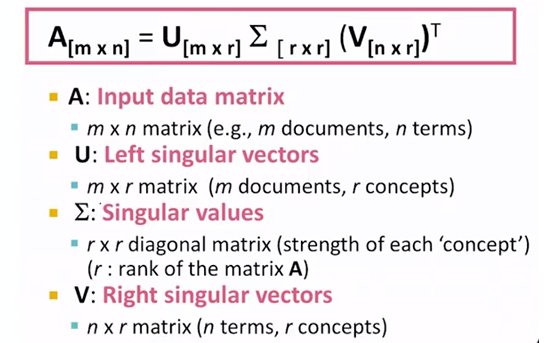
\includegraphics[width=0.6\linewidth,keepaspectratio]{svd4}
\end{center}
$V$ contains Eigen vectors and $\sum$ contains eigen values.
\end{frame}

%%%%%%%%%%%%%%%%%%%%%%%%%%%%%%%%%%%%%%%%%%%%%%%%%%%
\begin{frame}[fragile]
\frametitle{Singular Value Decomposition}
\begin{center}
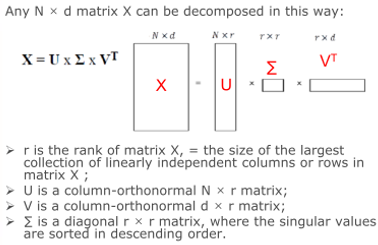
\includegraphics[width=0.8\linewidth,keepaspectratio]{svd1}
\end{center}
$V$ contains Eigen vectors and $\sum$ contains eigen values.
\end{frame}

%%%%%%%%%%%%%%%%%%%%%%%%%%%%%%%%%%%%%%%%%%%%%%%%%%%
\begin{frame}[fragile]
\frametitle{Singular Value Decomposition}
\begin{center}
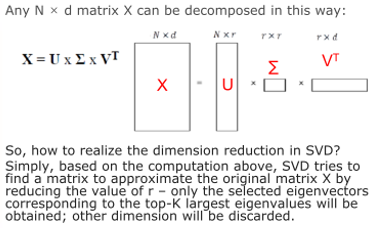
\includegraphics[width=0.8\linewidth,keepaspectratio]{svd3}
\end{center}
\end{frame}


%%%%%%%%%%%%%%%%%%%%%%%%%%%%%%%%%%%%%%%%%%%%%%%%%%%
\begin{frame}[fragile]
\frametitle{Singular Value Decomposition Properties}
\begin{center}
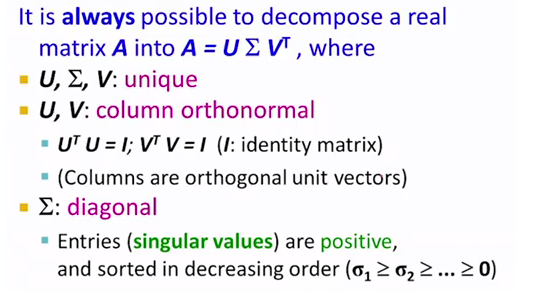
\includegraphics[width=\linewidth,keepaspectratio]{svd5}
\end{center}
\end{frame}



%%%%%%%%%%%%%%%%%%%%%%%%%%%%%%%%%%%%%%%%%%%%%%%%%%%
\begin{frame}[fragile]
\frametitle{Singular Value Decomposition}
\begin{center}
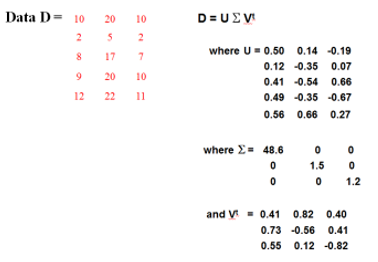
\includegraphics[width=0.8\linewidth,keepaspectratio]{svd2}
\end{center}
\end{frame}

%%%%%%%%%%%%%%%%%%%%%%%%%%%%%%%%%%%%%%%%%%%%%%%%%%%%%%%%%%%%%%%%%%%%%%%%%%%%%%%%%%
\begin{frame}[fragile]\frametitle{}
\begin{center}
{\Large Example - Movie Ratings}
\end{center}
\end{frame}

%%%%%%%%%%%%%%%%%%%%%%%%%%%%%%%%%%%%%%%%%%%%%%%%%%%
\begin{frame}[fragile]
\frametitle{Singular Value Decomposition Example}
Movie Ratings
\begin{center}
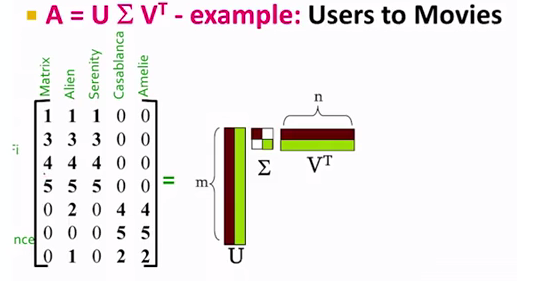
\includegraphics[width=0.8\linewidth,keepaspectratio]{svd6}
\end{center}
\tiny{(Reference: Dimensionality reduction: SVD and its applications - Viet-Trung TRAN)}
\end{frame}

%%%%%%%%%%%%%%%%%%%%%%%%%%%%%%%%%%%%%%%%%%%%%%%%%%%
\begin{frame}[fragile]
\frametitle{Singular Value Decomposition Example}
\begin{itemize}
	\item Some are Scifi movies, some romantic.
	\item SVD will try to figure this out.
	\item Matlab has ready SVD function
\end{itemize}

\begin{center}
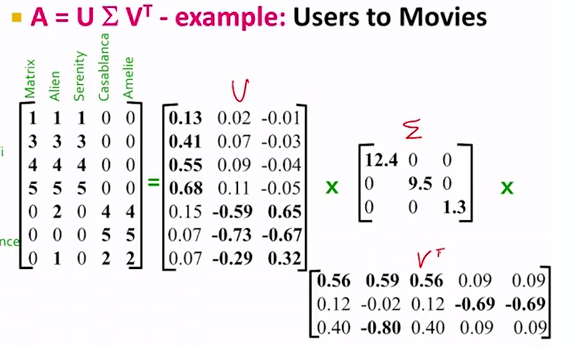
\includegraphics[width=0.8\linewidth,keepaspectratio]{svd7}
\end{center}
\end{frame}

%%%%%%%%%%%%%%%%%%%%%%%%%%%%%%%%%%%%%%%%%%%%%%%%%%%
\begin{frame}[fragile]
\frametitle{Singular Value Decomposition Example}
U matrix: User to Concepts distribution/matrix
\begin{itemize}

	\item Concepts as columns
	\item First few uses are more into Sci-fi
	\item First row: proportion of each column
\end{itemize}

\begin{center}
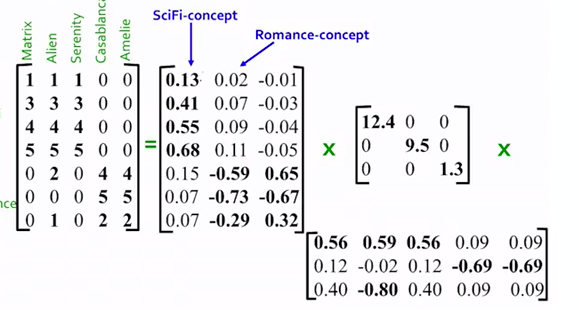
\includegraphics[width=0.8\linewidth,keepaspectratio]{svd8}
\end{center}
\end{frame}

%%%%%%%%%%%%%%%%%%%%%%%%%%%%%%%%%%%%%%%%%%%%%%%%%%%
\begin{frame}[fragile]
\frametitle{Singular Value Decomposition Example}
Sigma matrix
\begin{itemize}
	\item Strength of Scifi concept is more than other two
\end{itemize}

\begin{center}
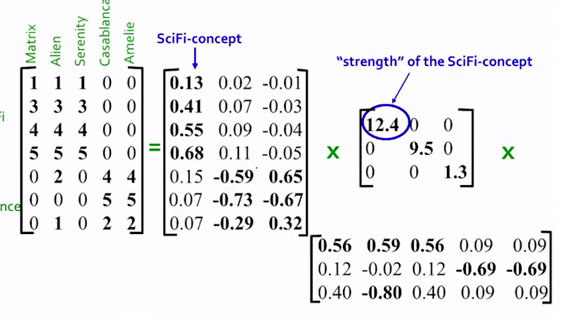
\includegraphics[width=0.8\linewidth,keepaspectratio]{svd9}
\end{center}
\end{frame}

%%%%%%%%%%%%%%%%%%%%%%%%%%%%%%%%%%%%%%%%%%%%%%%%%%%
\begin{frame}[fragile]
\frametitle{Singular Value Decomposition Example}
V matrix:  Concept to Movie matrix.
\begin{itemize}
	\item Scifi-ness in first few movies is more than others
\end{itemize}

\begin{center}
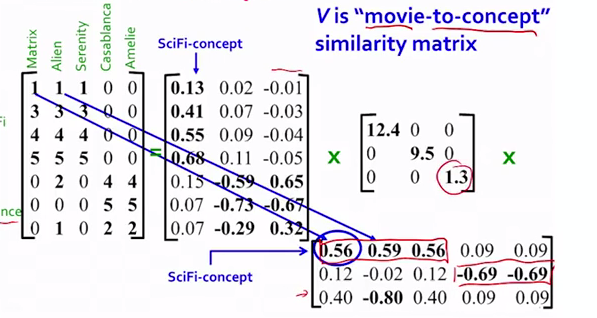
\includegraphics[width=0.8\linewidth,keepaspectratio]{svd10}
\end{center}
\end{frame}

